\section{Results}

The simulation was conducted in GPGPU-Sim for NVIDIA Fermi GPU
architecture \cite{bakhodayuan09}. 
GPGPU-Sim was configured to simulated the performance of
GTX580~\cite{gf100}, with all 16 streaming multiprocessors enabled
(each CUDA streaming multiprocessor is represented as a single SIMT
Core in GPGPU-Sim). 
Each streaming multiprocressor contains 48 warps, with 32 threads per
warp (See Figure \ref{GTX580}). 
All sixteen SIMT cores share unified L2 cache.

GPGPU-Sim~\cite{bakhodayuan09} is an open-source software package
available to simulate GPU architecture. 
It has been validated to be representative of performance on NVIDIA
GPUs and provides a reasonable platform for testing alternate
highly-parallel computer architectures.

\begin{figure}[ht!]
\centering
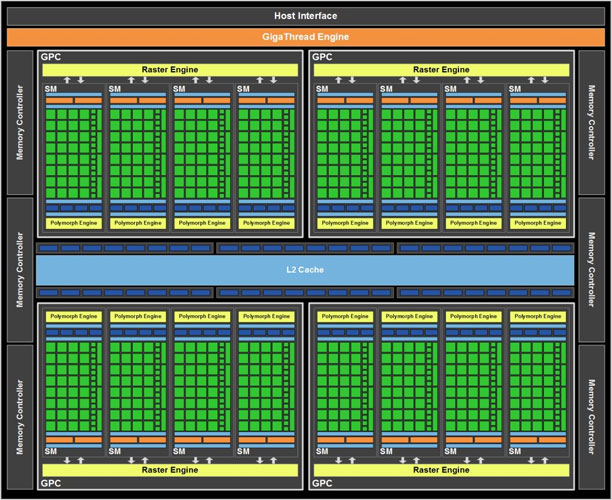
\includegraphics[width=\columnwidth]{graphics/GTX580.jpg}
\caption{Block Diagram of Default GTX580~\cite{gf100}. There are 16 SIMT Cores, all sharing a common L2 cache. Each SIMT Core contains a separate L1 cache.}
\label{GTX580}
\end{figure}

In the Fermi architecture, each streaming multiprocessor has
its own distinct L1 cache. 
Each L1 instruction cache is 4-way set associative, with 4 sets of
128 bytes per block. 
To assess the  performance of different L1 instruction cache
architectures, only the L1 instruction cache was modified, while all
other architectural variables remained constant. 
Other aspects of the architecture such as the bandwidth of shared L2
cache could serve as a performance bottleneck for different cache
designs. 
However, these variables are ignored for this study, because we expect
them to have little impact on the hit and stall rate of the
instruction cache, which are the primary metrics of interest.

\subsection{Projected Results}
\jbs{It isn't clear to me whether the following paragraph is
  theoretical results, or actual simulated results.}

The simulation results show two optimization
approaches in improving instruction cache performance by having
multiple GPU cores share the cache. 
One approach is to keep the total instruction cache size constant and
improve the performance of the cache, as shown in
Figure~\ref{HitImprov}. 
In this approach, when multiple cores are configured to share the same
instruction cache, the previous cache that existed with each core are
merged together to form larger caches. 
The increased sized of the cache may result in degredation in access
time, but improves the hit rate. 
The hit rate of the cache is expected to improve greatly when the size
of initial cache is doubled or tripled, but there will be less
improvement when the hit rate at a high level.


\begin{figure}[t]
\centering
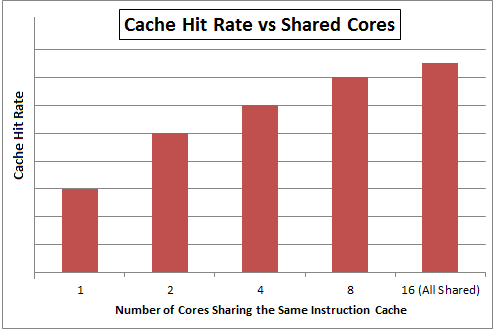
\includegraphics[width=\columnwidth]{graphics/HitRateImprov.png}
\caption{Projected Improvement in Hit Rate. Total size of the instruction cache remains constant. Size of individual instruction cache is scaled proportionally to the number of cores that share the cache.}
\label{HitImprov}
\end{figure}


\begin{figure}[b!]
\centering
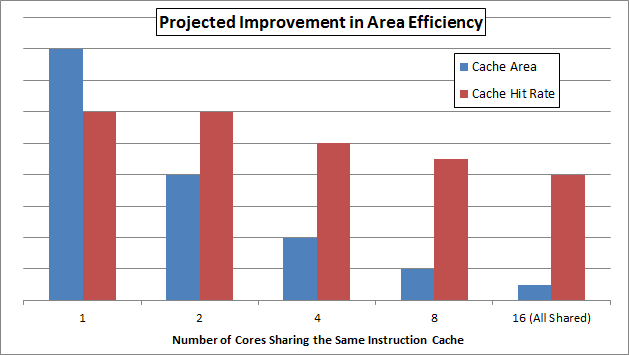
\includegraphics[width=\columnwidth]{graphics/AreaEff.png}
\caption{Projected Improvement in Area Efficiency. Size of individual instruction cache remains constant, while the number of cores sharing the L1 cache is increased. The instruction redundancy between the cores should allow cache hit rate to remain high as cache area is reduced. }
\label{AreaEff}
\end{figure}


The second approach is to reduce the total size of the cache by
keeping the size of individual instruction cache constant. 
In this approach, rather than merging the shared caches together, the
instruction caches are kept at the same size even if more cores are
sharing the same core. 
The hit rate of the cache may drop when the instruction cache is not
large enough to satisfy all the cores sharing the cache, but this drop
in hit rate is expected to be less than the reduction in area due to
the instruction redundancy between the shared cores.


\subsection{Benchmarks}
Describe benchmarks used \jbs{Akhil in charge.}

Several benchmark programs were used in this project. 
These benchmarks included STO, RAY, NQU, LPS, LIB, CP and BFS. 
In order to determine which of the aforementioned benchmarks would be
most useful for the purposes of our project, we performed an
experiment in which the performance of the benchmarks was examined as
a function of the number of cores used in the available GTX580
architecture. 
The number of cores was varied between 1 and 16 (the maximum number of
cores available on the GTX580). 
Then the miss and stall rate was noted for each different
architectural configuration. 
Figure \ref{fig:missStalls} shows the results of our experiment. 

\begin{figure}[b!]
\centering
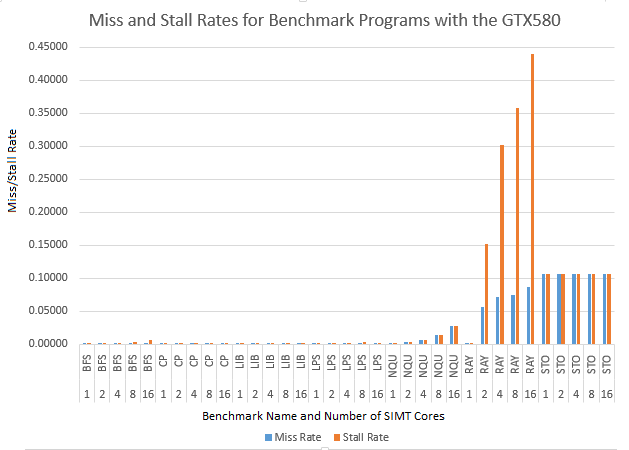
\includegraphics[width=\columnwidth]{graphics/miss_stalls_benchmarks.png}
\caption{Miss and Stall Rates for Benchmark Programs with the GTX580
\jbs{Are the numbers (1-4) the same here as for
  Figure~\ref{HitImprov}? Why is this miss rate when the others are
hit rate? We should unify the presentation.}
}
\label{fig:missStalls}
\end{figure}

\begin{figure}[b!]
\centering
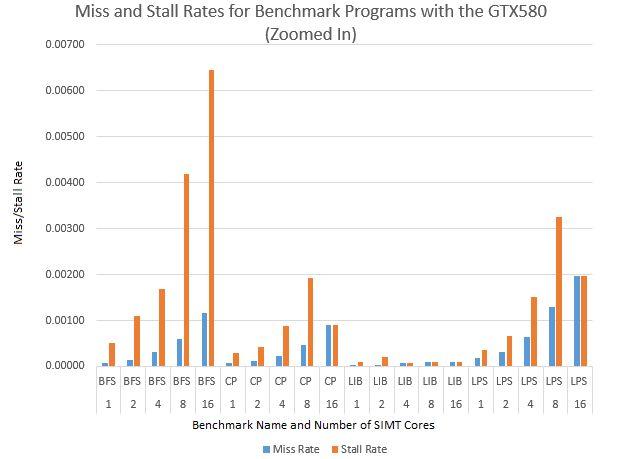
\includegraphics[width=\columnwidth]{graphics/miss_stalls_benchmarks_zoomed.png}
\caption{Miss and Stall Rates for Benchmark Programs with GTX580 (Zoomed In) }
\label{fig:missStallsZoomed}
\end{figure}

Figure \ref{fig:missStallsZoomed} is a zoomed in version of
\ref{fig:missStalls} included to enable better understanding of the
results with lower miss rates. 

The benchmark STO is mostly unaffected by this variation in the number of cores and RAY has a much higher
stall rate (indicating more reservation fails than misses) than its
miss rates, and is evidently more susceptible to the aforementioned change. 

RAY had more variability in how it was affected by the number of cores.

In order to explain the reasons behind the results shown in Figures
\ref{fig:missStalls} and \ref{fig:missStallsZoomed}, we examined the
degree of parallelism of RAY and CP.

The degree of parallelism is a representation of the number of software
work elements that each program issues to the GPU when executing in
hardware. 
Calculations on the number of issued work elements is a representation of the level of parallelism employed by
2 programs which we found interesting as per our previous results.

\emph{CP (Coulombic Potential)}

Given a standard configuration, CP issues a high number of thread blocks -- a representation of the high degree of parallelism that CP takes advantage of.

The reason only the parallelism of CP and RAY were examined was that
from a preliminary inspection, they seemed to having a desired
combination of parallelism and size of instruction set. 

From all the aforementioned results, it was clear that RAY was the
most interesting bechmark. 
This was because it had the highest number of PTX instructions issued
and was also significatly parallel. 
Moreover, the fact that the degree of parallelism of RAY could be
increased easily by modifying the CUDA program, we nominated RAY as
our most significant benchmark program.
 
Increasing the degree of parallelism in software entailed changing the
image size that the Ray Tracer would operate on.
 
By increasing the size of the picture to 512 by 512, we made RAY issue a much higher number of thread blocks per unit time. 

This ensured that the RAY benchmark was executing as parallel in
software as the Coulombic Potential benchmark in the number of work
elements that it was issuing. 
Given that the RAY CUDA file issues more instructions in its core
computation that CP does, and that a lot of its instructions (CUDA
instructions) seem to be computationally more expensive, RAY can now
be treated as both a long program which would occupy a significant
amount of space in the instruction cache (and hence would not be
entirely resident in the instruction cache) AND would issue those
instructions with a high degree of parallelism.

\subsection{Preliminary Results}
\jbs{Fabiha in charge}

The performed simulations point to several factors that may account 
for the outcomes seen with each approach. Parameters that are expected 
to affect instruction cache performance include the number of cores 
shared, associativity, parallelism, and cache size.

The first method, varying the number of cores sharing a cache while 
keeping the total cache size constant, was expected to improve the hit 
rate. As the number of cores sharing the cache increased, the miss rate 
and stall rate both increased, with the later increasing more rapidly 
due to the higher number of reservation fails. While the hit rate may 
have improved, there was an overall trend of increased reservation fails 
because the cache was preoccupied with instructions from the greater 
number of cores. As an exception to this, CP demonstrated a balance as 
the stall rate decreased going from 8 cores to 16 cores sharing the 
cache. This was most likely due to the higher level of parallelism that 
CP had in comparison to the other benchmarks. Meanwhile, smaller programs 
remained unaffected more often than larger benchmarks.

The second approach entailed reducing the total cache size by keeping 
the size of each individual instruction cache constant when merging the 
cores that share each one. The reduction in area of the now shared cache 
allowed duplicate instructions to be accessed more quickly. This 
affected benchmarks with many reused instructions and is expected to 
provide space to be used for other caches.

Overall, these methods appear to perform best on multi-threaded 
applications with many reused instructions. Meanwhile, for benchmarks 
with higher hit rates to begin with, and thus less reservation fails, 
this method made less of an impact.
